\chapter{Architettura del Sistema}
\label{cap:ProgettazioneRealizzazione}

\emph{In questo capitolo verranno descritte le scelte architetturali
adottate per estendere la piattaforma Serverledge con le componenti
necessarie a una schedulazione carbon-aware. Verranno presentati il
modello di funzione logica con varianti, l'integrazione di Kepler per
il monitoraggio dei consumi a livello di container, il meccanismo di
aggiornamento adattivo dei profili energetici tramite media mobile
esponenziale e il meccanismo di esplorazione LCB per il raffinamento
delle stime nelle fasi iniziali. Lo scheduler che utilizza queste
componenti per la selezione carbon-aware delle varianti è oggetto del
Capitolo~\ref{cap:scheduler}.}
\section{Integrazione di Kepler per il monitoraggio energetico}

Il monitoraggio dei consumi energetici a livello di container costituisce 
il fondamento del sistema realizzato. A tal fine è stato adottato Kepler 
(Kubernetes-based Efficient Power Level Exporter), uno strumento open 
source sviluppato nell'ambito della CNCF (Cloud Native Computing 
Foundation) che stima il consumo energetico di processi, container e 
pod Kubernetes attraverso l'accesso diretto alle interfacce hardware del 
sistema operativo host~\cite{keplerCNCF2023}.

La scelta di Kepler è motivata principalmente dalla sua granularità di 
misurazione, che opera a livello di singolo container Docker: questa 
corrisponde esattamente all'unità di esecuzione delle funzioni serverless 
in Serverledge. Kepler espone inoltre le proprie metriche nel formato 
standard Prometheus, consentendo un'integrazione diretta con l'ecosistema 
di monitoraggio senza richiedere componenti aggiuntivi per la raccolta 
dei dati.

\subsection{Funzionamento di Kepler}

Kepler opera combinando due meccanismi complementari per associare i 
consumi energetici ai singoli container. Il primo è un programma eBPF 
(Extended Berkeley Packet Filter) integrato nel kernel, che traccia 
l'attività dei processi e li associa ai container tramite il file 
\texttt{/proc/PID/cgroup}, consentendo di correlare il Process ID di 
ciascun processo all'identificatore del container che lo ospita. Il 
secondo è l'interfaccia RAPL (Running Average Power Limit), disponibile 
sui processori Intel e AMD moderni, che permette di leggere i contatori 
energetici cumulativi direttamente dai registri hardware della CPU.

Una volta raccolti i dati di utilization dei processi e di consumo 
energetico del sistema, Kepler applica il \emph{Ratio Power Model} per 
attribuire a ciascun container la propria quota di consumo: la potenza 
dinamica viene distribuita tra i container in proporzione alla loro 
utilization rispetto all'utilization totale del sistema. Il risultato 
viene aggregato a livello di container e reso disponibile tramite 
Prometheus nella metrica \texttt{kepler\_container\_cpu\_joules\_total}, 
un contatore cumulativo espresso in Joule che cresce monotonicamente nel 
tempo per ogni container attivo.

\begin{figure}[ht]
    \centering
    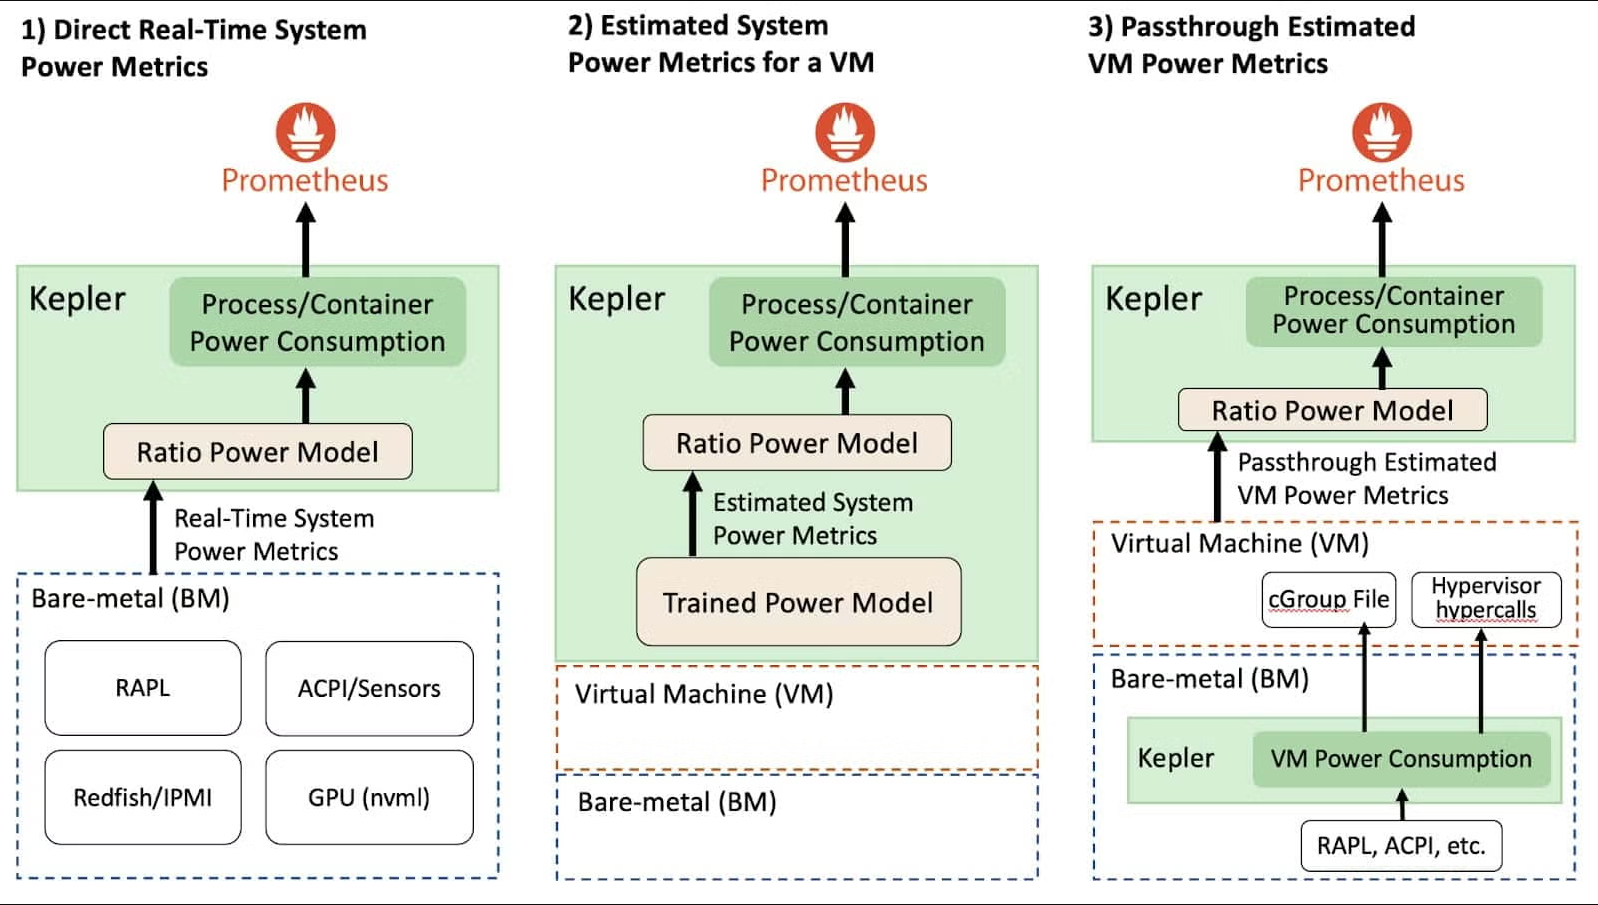
\includegraphics[width=0.85\textwidth]{figures/KeplerArchitecture.jpg}
    \caption{Architettura di Kepler per la raccolta dei consumi energetici 
    in ambienti bare-metal e virtuali. In ambienti bare-metal, Kepler 
    accede direttamente ai contatori hardware tramite RAPL, ottenendo 
    misurazioni real-time senza necessità di modelli predittivi. }
    \label{fig:kepler-arch}
\end{figure}

Come illustrato in Figura~\ref{fig:kepler-arch}, il comportamento di
Kepler varia in base all'ambiente di esecuzione. In ambienti bare-metal,
Kepler accede direttamente ai contatori RAPL, ottenendo misurazioni
energetiche real-time senza ricorrere a modelli predittivi
pre-addestrati. In ambienti virtualizzati, invece, l'assenza di accesso
diretto all'hardware richiede l'uso di modelli di regressione,
introducendo le relative limitazioni di accuratezza.

Per accedere alle interfacce hardware necessarie, Kepler deve essere 
eseguito con privilegi elevati sull'host: richiede accesso a 
\texttt{/sys} e \texttt{/proc} per leggere i contatori RAPL e i cgroup, 
e al socket Docker per identificare i container attivi e associarvi le 
metriche energetiche.

\subsection{Infrastruttura di supporto}

L'avvio dell'infrastruttura di monitoraggio è gestito dallo script 
\texttt{StartMetrics.sh}, che inizializza come container Docker tutti 
i servizi necessari al funzionamento del sistema.  
\begin{figure}[H]
    \centering
    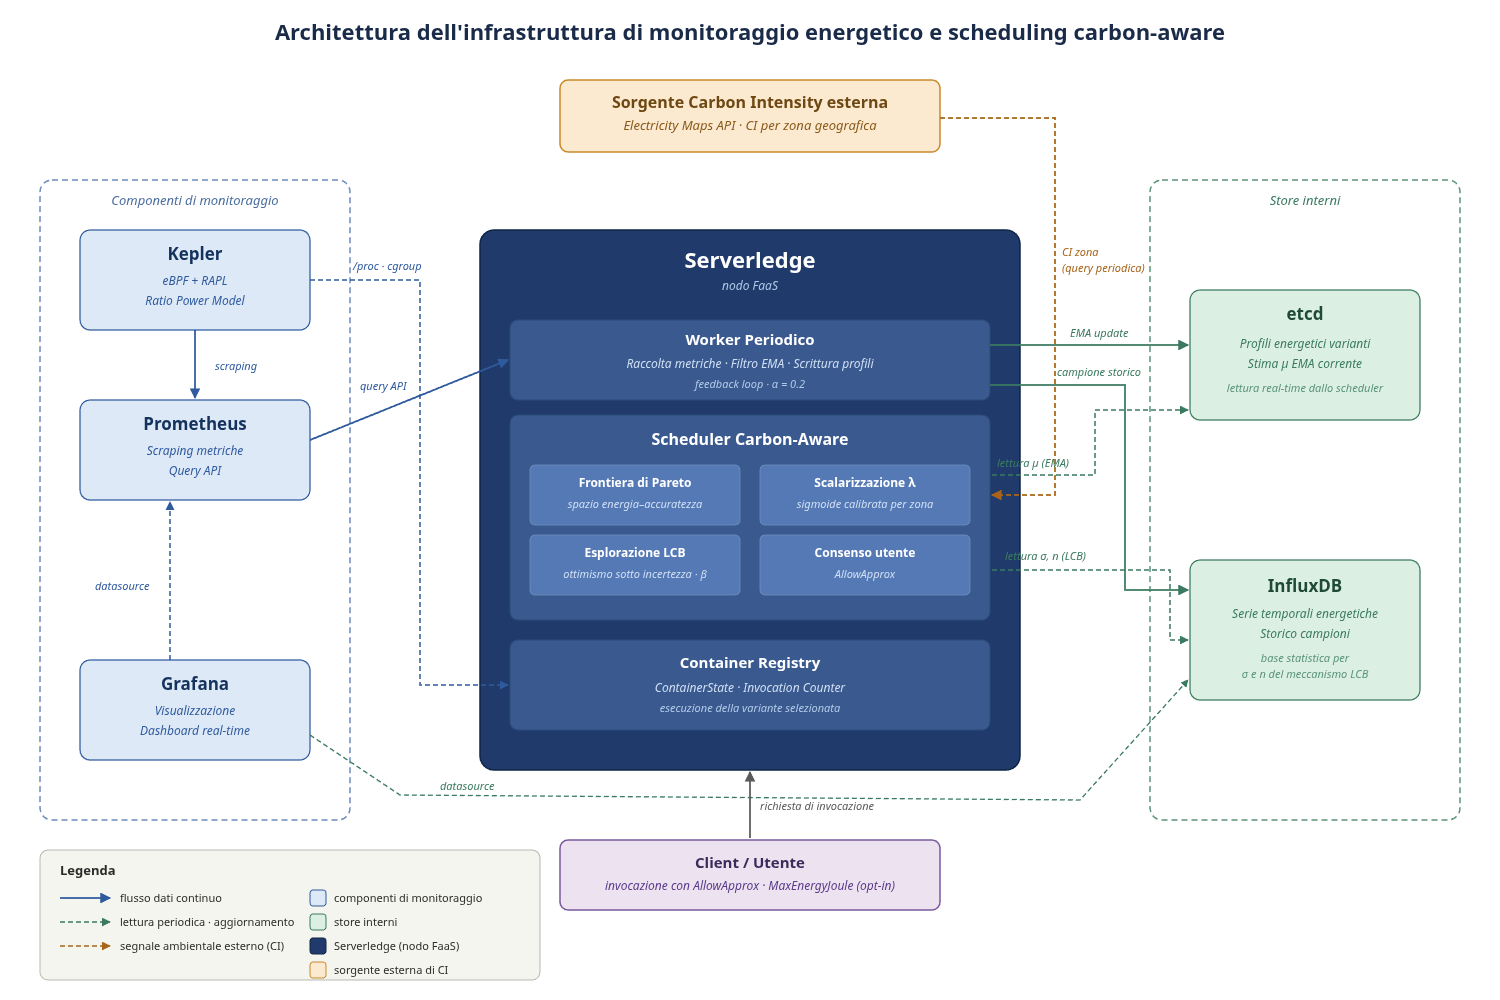
\includegraphics[width=0.85\textwidth]{figures/infrastracture-diagram.png}
    \caption{Architettura dell'infrastruttura di monitoraggio energetico e scheduling
carbon-aware. I componenti di monitoraggio esterni (Kepler, Prometheus, Grafana)
sono separati dagli store interni (etcd, InfluxDB), con Serverledge al centro
che interagisce con entrambi i livelli. Lo scheduler carbon-aware integra la
logica di selezione della variante — basata su frontiera di Pareto, scalarizzazione
tramite $\lambda$, esplorazione LCB e consenso utente — e riceve il segnale di
carbon intensity tramite query periodica a una sorgente esterna.}
    \label{fig:infra-arch}
\end{figure}

I componenti avviati,  come mostrato anche in Figura~\ref{fig:infra-arch}, sono i seguenti:

\begin{itemize}
    \item \textbf{Kepler}: eseguito in modalità privilegiata con accesso
 a \texttt{/sys}, \texttt{/proc} e al socket Docker dell'host, 
    condizioni necessarie per la lettura dei contatori RAPL e 
    l'associazione dei consumi ai container tramite cgroup.
    
    \item \textbf{Prometheus}: configurato per effettuare lo scraping 
    periodico delle metriche esposte da Kepler, rendendole disponibili 
    tramite API di interrogazione.
    
    \item \textbf{InfluxDB}: database a serie temporali utilizzato per 
    l'archiviazione storica dei campioni energetici prodotti dal 
    sistema ad ogni ciclo di raccolta.
    
    \item \textbf{etcd}: store distribuito chiave-valore che funge da 
    registro delle funzioni e delle relative varianti, inclusi i profili 
    energetici aggiornati dinamicamente a runtime.
    
    \item \textbf{Grafana}: strumento di visualizzazione utilizzato per 
    il monitoraggio in tempo reale dei consumi durante gli esperimenti.
\end{itemize}

Una volta avviata, l'infrastruttura opera in modo autonomo: Kepler 
rileva i container Docker presenti sull'host e ne aggiorna le metriche 
energetiche ad ogni ciclo di campionamento; Prometheus le raccoglie e 
le rende interrogabili; il sistema interno di Serverledge, descritto nelle sezioni successive,
le legge periodicamente --- limitatamente ai container attivi da esso gestiti --- per aggiornare i profili energetici 
delle varianti di funzione. Il segnale di carbon intensity, necessario allo scheduler 
per la selezione carbon-aware della variante, non è parte di questa infrastruttura: 
viene acquisito dallo scheduler a runtime tramite query periodica a una 
sorgente esterna, come descritto nella Sezione~\ref{cap:scheduler}.
\section{Il modello di funzione logica con varianti}
\label{sec:variant-model}

Il supporto all'esecuzione energeticamente consapevole richiede che il 
sistema possa rappresentare, per una stessa funzione, implementazioni 
alternative con diversi profili di consumo e accuratezza. A tal fine è 
stato introdotto il concetto di \emph{funzione logica con varianti}: 
un'astrazione che raggruppa sotto un unico identificatore logico più 
implementazioni della stessa funzione, ciascuna caratterizzata da un 
proprio profilo energetico e da un modello di output che ne quantifica 
l'accuratezza.

\subsection{Struttura della funzione e profilo energetico}

In Serverledge, ogni funzione è rappresentata dalla struttura 
\texttt{Function}, estesa in questo lavoro con i campi necessari al 
supporto delle varianti energetiche. I campi rilevanti per il sistema 
proposto sono i seguenti:

\begin{itemize}
    \item \texttt{LogicalName}: identificatore condiviso da tutte le 
    varianti appartenenti alla stessa funzione logica. Costituisce 
    il riferimento con cui il client invoca la funzione, 
    indipendentemente dalla variante che verrà selezionata a runtime.

    \item \texttt{VariantID}: identificatore univoco della specifica 
    variante all'interno del gruppo logico (ad esempio \texttt{base}, 
    \texttt{light}, \texttt{c}).

    \item \texttt{EnergyProfile}: struttura che mantiene la stima 
    energetica della variante, composta da due campi:
    \begin{itemize}
        \item \texttt{ColdStartJoule}: energia stimata per l'avvio a 
        freddo del container, comprensiva dell'inizializzazione del 
        runtime;
        \item \texttt{InvocationJoule}: energia media stimata per una 
        singola invocazione della funzione
    \end{itemize}
    \item \texttt{AllowApprox}: flag booleano che indica se la funzione 
    logica ammette l'utilizzo di varianti approssimate. La sua 
    attivazione è condizione necessaria affinché lo scheduler 
    energy-aware possa considerare varianti con accuratezza ridotta.
\end{itemize}

\subsubsection{Determinazione dei profili energetici iniziali}

I valori iniziali di \texttt{EnergyProfile} sono stati determinati 
offline tramite una campagna di misurazioni preliminari condotta con 
Kepler. La metodologia adottata tiene conto della natura delle metriche 
esposte da Kepler: trattandosi di contatori cumulativi, l'energia 
osservata al termine di $n$ invocazioni consecutive sullo stesso 
container rappresenta la somma dei contributi di tutte le esecuzioni, 
inclusa quella iniziale soggetta al cold start.

Per separare i due contributi energetici si è proceduto nel modo 
seguente. Dato un container su cui vengono eseguite $n$ invocazioni 
consecutive, si indica con $E_{tot}$ l'energia cumulativa totale 
rilevata da Kepler al termine dell'ultima invocazione e con $E_1$ 
l'energia della prima invocazione, che comprende sia il costo di 
inizializzazione del container che quello di esecuzione della funzione. 
Le invocazioni successive, eseguite a container già attivo, sono invece 
soggette al solo costo di esecuzione. Il costo medio di invocazione in 
warm start è quindi stimato come:

\begin{equation}
    E_{inv} = \frac{E_{tot} - E_1}{n - 1}
    \label{eq:inv-joule}
\end{equation}

e il costo di cold start come:

\begin{equation}
    E_{cold} = E_1 - E_{inv}
    \label{eq:cold-joule}
\end{equation}

La ripetizione delle misurazioni su un numero statisticamente 
significativo di invocazioni consente di attenuare la varianza 
introdotta dal sistema operativo e dal runtime, ottenendo stime 
robuste per entrambi i contributi. I valori così ottenuti vengono 
codificati nel file JSON di definizione delle varianti e costituiscono 
la stima iniziale del profilo energetico. Il \autoref{lst:fibonacci-json} 
mostra un esempio concreto per la funzione \texttt{fibonacci}, che 
espone tre varianti con profili energetici distinti.

\begin{lstlisting}[
    language=json,
    caption={File di definizione delle varianti per la funzione 
    \texttt{fibonacci}. Ciascuna variante specifica runtime, entry 
    point, profilo energetico iniziale e modello di output.},
    label={lst:fibonacci-json}
]
{
  "variants": [
    {
      "id": "base",
      "runtime": "python310",
      "entry_point": "fibonacci.handler",
      "src": "fibonacci.py",
      "energy": {
        "cold_start_joule": 0.06606,
        "invocation_joule": 0.000731579
      },
      "output": { "type": "error", "error_estimate": 0.0 },
      "is_approximate": false
    },
    {
      "id": "optimization-py",
      "runtime": "python310",
      "entry_point": "fibonacci_o.handler",
      "src": "fibonacci_o.py",
      "energy": {
        "cold_start_joule": 0.05640,
        "invocation_joule": 0.000494737
      },
      "output": { "type": "error", "error_estimate": 0.0 },
      "is_approximate": false
    },
    {
      "id": "c",
      "runtime": "native",
      "entry_point": "fibonacci",
      "src": "fibonacci",
      "energy": {
        "cold_start_joule": 0.008268422,
        "invocation_joule": 0.000171579
      },
      "output": { "type": "error", "error_estimate": 0.0 },
      "is_approximate": false
    }
  ]
}
\end{lstlisting}

I valori iniziali del profilo energetico sono progressivamente 
raffinati a runtime dal worker periodico, che aggiorna entrambi i valori sulla base delle misurazioni effettive 
raccolte durante l'esecuzione in produzione. I risultati numerici 
delle misurazioni preliminari per tutte le varianti sono riportati 
nel Capitolo~\ref{cap:RisultatiSperimentali}.
\subsection{Il modello di output e la classificazione dell'accuratezza}
\label{sec:output-model}

Per consentire allo scheduler di confrontare le varianti in termini di 
accuratezza, ciascuna variante è dotata di un \texttt{OutputModel} che 
descrive la qualità del suo output. Il modello supporta due tipologie 
di classificazione, scelte in base alla natura computazionale della 
funzione:

\begin{itemize}
    \item \textbf{Tipo \texttt{error}}: adatto a funzioni il cui output 
    è un valore numerico misurabile. L'accuratezza è espressa tramite 
    il campo \texttt{error\_estimate}, che rappresenta l'errore relativo 
    atteso rispetto alla variante di riferimento. Una variante esatta 
    presenta \texttt{error\_estimate = 0.0}, mentre varianti approssimate 
    presentano valori positivi proporzionali alla deviazione introdotta 
    dalla semplificazione algoritmica adottata.

    \item \textbf{Tipo \texttt{quality}}: adatto a funzioni il cui 
    output non è facilmente quantificabile con un errore numerico, 
    come classificatori o modelli di machine learning. L'accuratezza 
    è espressa tramite un livello discreto: \texttt{high}, 
    \texttt{medium} o \texttt{low}, che riflette la qualità complessiva 
    del risultato prodotto dalla variante.
\end{itemize}

Il ~\autoref{lst:imageclassification-json} mostra un esempio 
applicativo del tipo \texttt{quality} per la funzione 
\texttt{ImageClassification}, in cui la variante base utilizza un 
modello di rete neurale più accurato ma più oneroso, mentre la 
variante \texttt{Light} adotta un modello più compatto a qualità ridotta.

\begin{lstlisting}[
    language=json,
    caption={File di definizione delle varianti per la funzione 
    \texttt{ImageClassification}. Il campo \texttt{quality} esprime 
    l'accuratezza in forma discreta, adatta a output non numericamente 
    quantificabili.},
    label={lst:imageclassification-json}
]
{
  "variants": [
    {
      "id": "base",
      "runtime": "python-ml",
      "entry_point": "ImageClassification.handler",
      "src": "ImageClassification.py",
      "energy": {
        "cold_start_joule": 1.894736842,
        "invocation_joule": 1.455263158
      },
      "output": { "type": "quality", "quality": "high" },
      "is_approximate": false
    },
    {
      "id": "Light",
      "runtime": "python-ml",
      "entry_point": "ImageClassificationLight.handler",
      "src": "ImageClassificationLight.py",
      "energy": {
        "cold_start_joule": 1.071052329,
        "invocation_joule": 0.22894768
      },
      "output": { "type": "quality", "quality": "low" },
      "is_approximate": true
    }
  ]
}
\end{lstlisting}

Lo scheduler converte internamente entrambe le rappresentazioni in un 
punteggio numerico (\emph{ErrorScore}) secondo una scala uniforme: 
per il tipo \texttt{error} viene utilizzato direttamente il valore di 
\texttt{error\_estimate}, mentre per il tipo \texttt{quality} i livelli 
\texttt{high}, \texttt{medium} e \texttt{low} vengono mappati 
rispettivamente a $0.0$, $1.0$ e $2.0$. La selezione privilegia 
sempre la variante con il punteggio più basso compatibile con il 
vincolo energetico, garantendo che la qualità del risultato sia 
massimizzata nei limiti imposti dalla richiesta.

La Tabella~\ref{tab:output-models} riassume il modello di output 
adottato per ciascuna delle funzioni utilizzate negli esperimenti.

\begin{table}[h]
    \centering
    \begin{tabular}{llll}
        \toprule
        \textbf{Funzione} & \textbf{Tipo} & 
        \textbf{Variante base} & \textbf{Variante approssimata} \\
        \midrule
        Fibonacci         & \texttt{error}   & 0.0  & 0.0 \\
        PiLeibniz         & \texttt{error}   & 0.0  & $1.99 \times 10^{-8}$ \\
        Sqrt              & \texttt{error}   & 0.0  & 0.043 \\
        VectorMagnitude   & \texttt{error}   & 0.0  & 0.04 \\
        SentimentAnalysis & \texttt{quality} & high & low \\
        ImageClassification & \texttt{quality} & high & low \\
        \bottomrule
    \end{tabular}
    \caption{Modello di output adottato per ciascuna funzione. Per il 
    tipo \texttt{error} il valore riportato è \texttt{error\_estimate}; 
    per il tipo \texttt{quality} il livello discreto assegnato.}
    \label{tab:output-models}
\end{table}
\subsection{Registrazione e indicizzazione delle varianti in etcd}
\label{sec:variant-registration}

Le varianti di una funzione logica vengono definite tramite un file 
JSON collocato nella directory \texttt{variants/<LogicalName>/} del 
progetto. Al momento della registrazione, il sistema legge questo file 
attraverso il componente \texttt{FileSource}, prepara il codice 
sorgente di ciascuna variante in formato tar e materializza le varianti 
in etcd attraverso la funzione \texttt{CreateInternalVariants}.

\subsubsection{Convenzione di denominazione}

La convenzione di denominazione distingue la variante di riferimento 
dalle varianti alternative. La prima variante definita nel file JSON, tipicamente quella a massima accuratezza, mantiene come nome interno 
esattamente il \texttt{LogicalName}, preservando la compatibilità con 
le invocazioni che non specificano alcuna preferenza energetica. Le 
varianti successive ricevono un nome composto nella forma 
\texttt{<LogicalName>-<VariantID>}. Per la funzione logica 
\texttt{fibonacci} (\autoref{lst:fibonacci-json}) ad esempio, i nomi interni assegnati sono:

\begin{itemize}
    \item \texttt{fibonacci} — variante base in Python
    \item \texttt{fibonacci-optimization-py} — variante ottimizzata 
    in Python
    \item \texttt{fibonacci-c} — variante compilata in C nativo
\end{itemize}

\subsubsection{Struttura delle chiavi in etcd}

Il sistema mantiene in etcd due livelli distinti di chiavi, ciascuno 
con una responsabilità specifica, come illustrato in 
Figura~\ref{fig:etcd-structure}.

Il primo livello, sotto il prefisso \texttt{/function/}, contiene una 
chiave per ogni variante registrata nel sistema, indipendentemente 
dalla funzione logica di appartenenza. Il valore associato è la 
serializzazione JSON completa della struttura \texttt{Function}, che 
include il runtime, il codice sorgente, il profilo energetico corrente 
e il modello di output. È su queste chiavi che il worker periodico 
scrive gli aggiornamenti del campo \texttt{InvocationJoule} ad ogni 
ciclo di raccolta.

Il secondo livello, sotto il prefisso 
\texttt{/index/logical/<LogicalName>/}, costituisce un indice che 
associa ciascun nome logico all'insieme delle sue varianti. La 
motivazione di questo indice è di natura prestazionale: poiché la 
selezione della variante avviene nel critical path della richiesta di 
invocazione, è necessario che lo scheduler possa recuperare 
rapidamente tutte le varianti di una funzione logica senza dover 
scorrere l'intero prefisso \texttt{/function/}, che contiene tutte 
le funzioni registrate nel sistema. Tramite l'indice, il recupero 
avviene con una singola query con prefisso su 
\texttt{/index/logical/<LogicalName>/}, restituendo esclusivamente le 
varianti della funzione richiesta e contenendo così la latenza 
introdotta dalla fase di selezione a runtime.

\begin{figure}[H]
    \centering
    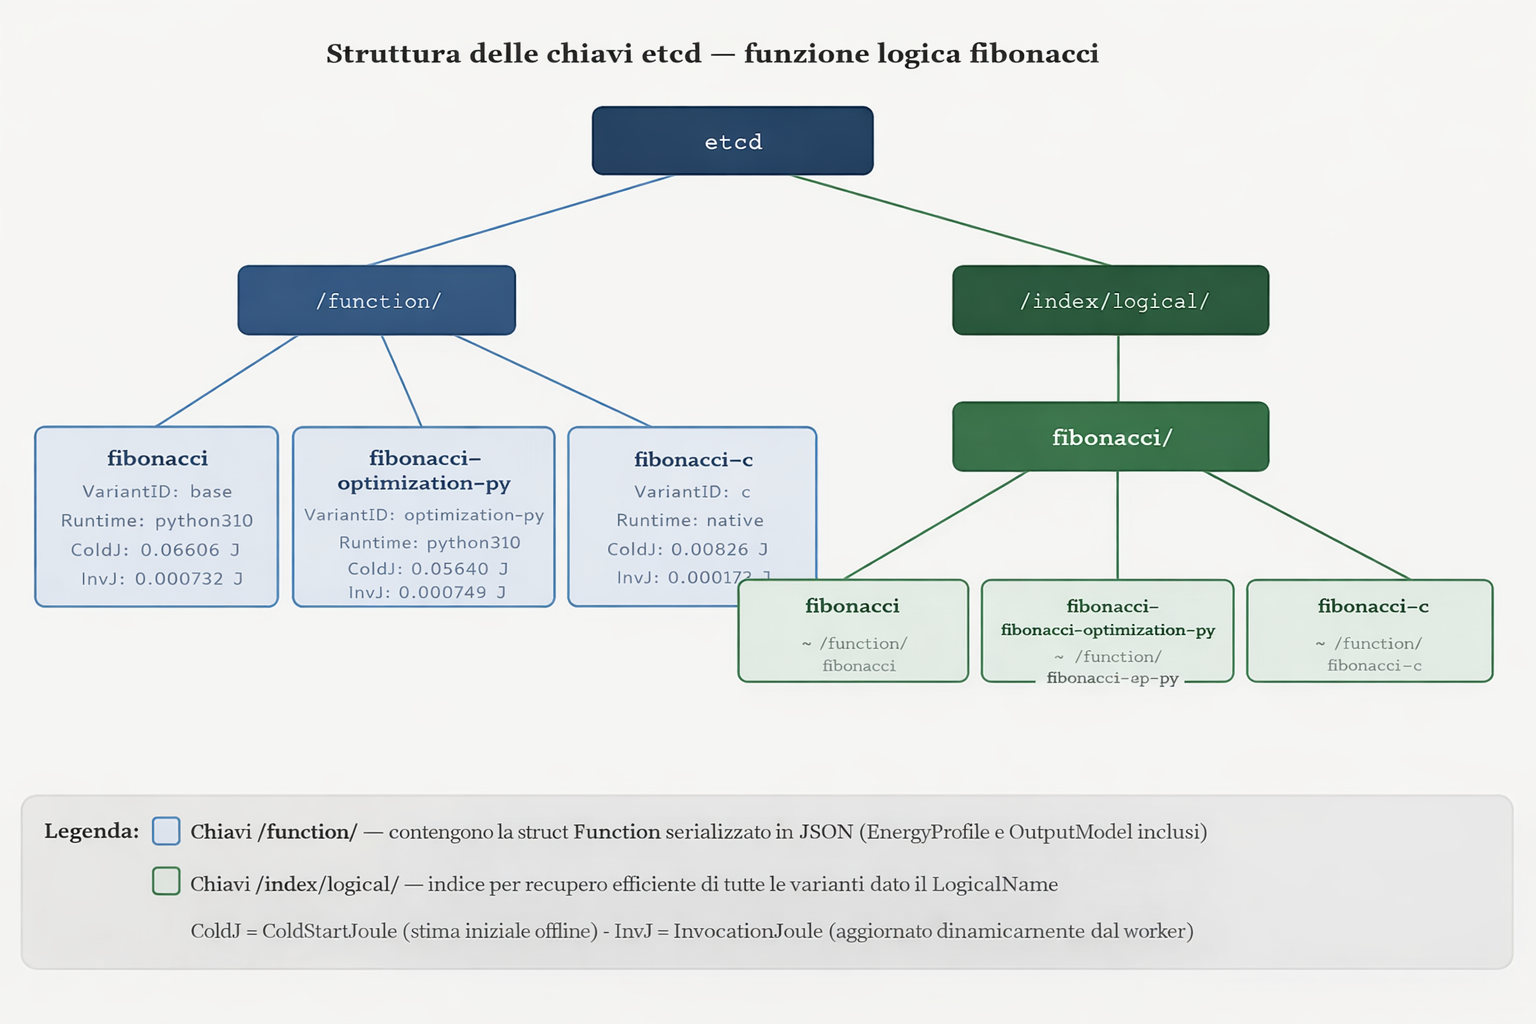
\includegraphics[width=0.95\textwidth]{figures/etcd-structure.jpg}
    \caption{Struttura delle chiavi etcd per la funzione logica 
    \texttt{fibonacci} con tre varianti. Le chiavi sotto 
    \texttt{/function/} contengono i profili completi aggiornati dal 
    worker periodico. L'indice sotto \texttt{/index/logical/} consente 
    allo scheduler di recuperare efficientemente le sole varianti della 
    funzione richiesta, senza scorrere l'intero store.}
    \label{fig:etcd-structure}
\end{figure}
\section{Misurazione e aggiornamento adattivo dei profili energetici}
\label{sec:worker}

Una volta introdotto il modello di funzione logica con varianti multiple,
è necessario dotare il sistema di un meccanismo capace di aggiornare
dinamicamente i profili energetici sulla base dei consumi effettivamente
osservati a runtime. Un approccio statico, in cui il costo energetico di
una variante viene stimato offline e rimane invariato nel tempo, risulta
inadeguato in contesti di esecuzione reali: il consumo energetico di un
container è influenzato da fattori mutevoli quali il carico del nodo,
le interferenze tra istanze concorrenti e le variazioni dinamiche della
frequenza di CPU.

La soluzione adottata è un \emph{feedback loop} periodico che trasforma
il profilo energetico in una grandezza adattiva, aggiornata continuamente
in funzione del contesto di esecuzione. Il componente responsabile è un
worker di raccolta eseguito in background, illustrato in
Figura~\ref{fig:worker-architecture}.

\begin{figure}[ht]
    \centering
    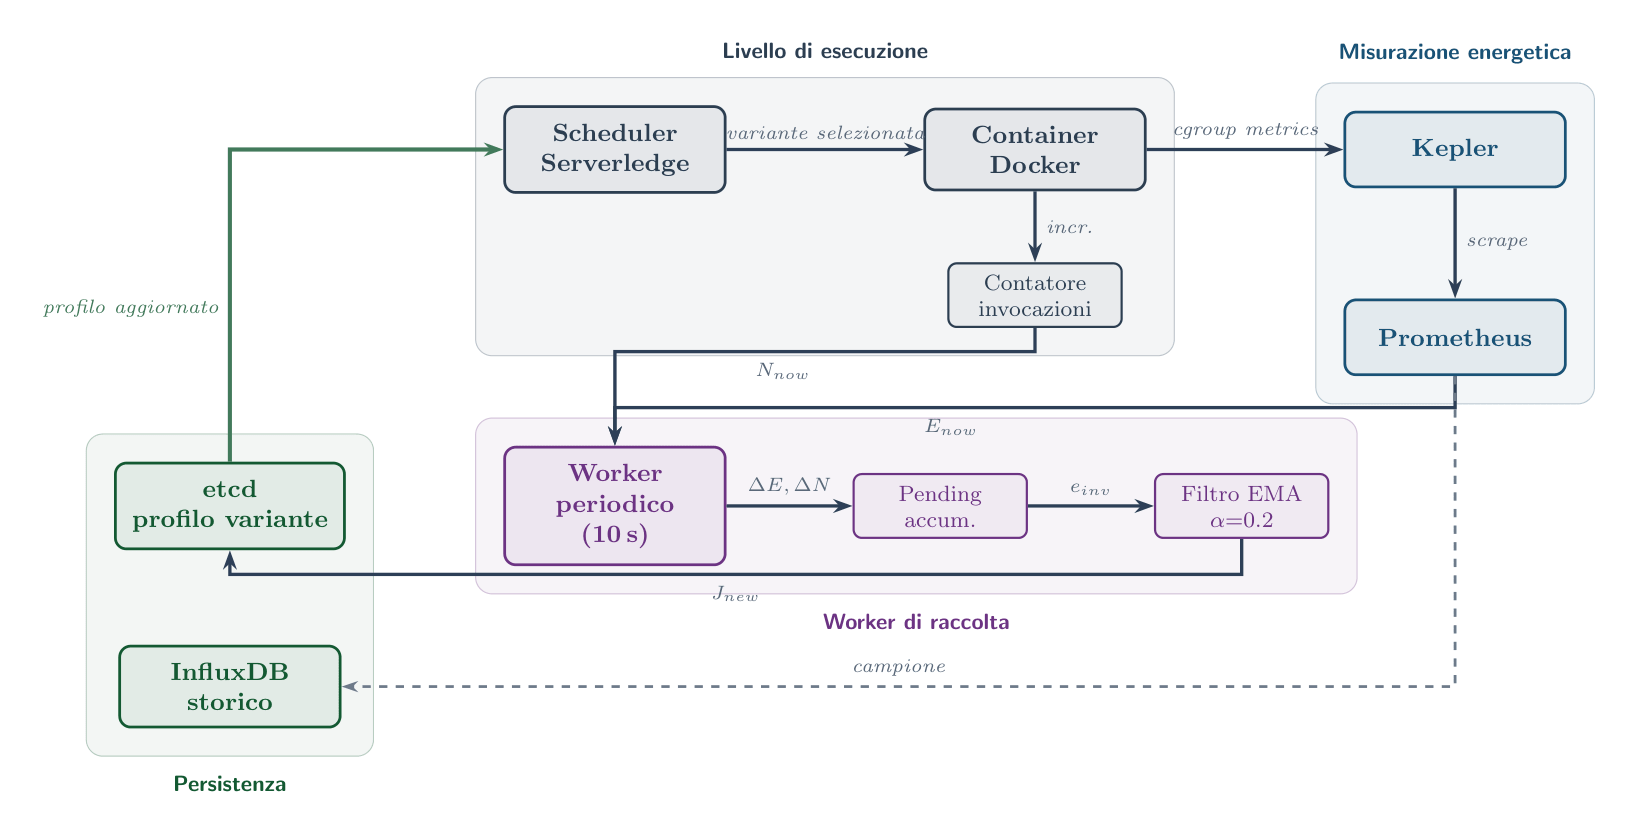
\includegraphics[width=\textwidth]{figures/Worker.png}
    \caption{Schema del feedback loop energetico. Il worker periodico
    legge le metriche cumulative da Kepler tramite Prometheus e il numero
    di invocazioni dal contatore locale, calcola i delta, applica un
    filtro EMA e aggiorna il profilo persistito in etcd, archiviando
    contestualmente i campioni in InfluxDB.}
    \label{fig:worker-architecture}
\end{figure}


\subsection{Tracciamento dei container e conteggio delle invocazioni}
\label{subsec:container-registry}

Per attribuire correttamente il consumo energetico alle singole varianti,
il sistema deve mantenere una corrispondenza stabile tra i container
Docker attivi e le funzioni in esecuzione. A tal fine il package
\texttt{energy} mantiene un registro in memoria che associa a ciascun
container una struttura \texttt{ContainerState} contenente:

\begin{itemize}
    \item l'identificatore del container (\texttt{ContainerID});
    \item il nome interno della variante (\texttt{FunctionName}), il
    \texttt{LogicalName} e il \texttt{VariantID};
    \item i valori di baseline dell'energia cumulativa e del numero di
    invocazioni (\texttt{LastJoule}, \texttt{LastInvocations}),
    impiegati per il calcolo dei delta incrementali;
    \item gli accumulatori \texttt{PendingEnergyJ} e
    \texttt{PendingInvocations}, necessari per gestire il disallineamento
    temporale tra metriche energetiche e contatori locali.
\end{itemize}

La registrazione avviene sia alla creazione del container sia, in modo
difensivo, al momento dell'invocazione, così da gestire correttamente il
caso di \emph{warm start}. Se un container è già presente nel registro,
la sua identità (mapping container-variante) non viene modificata,
garantendo coerenza per l'intero ciclo di vita del container.

Parallelamente, viene mantenuto un contatore atomico di invocazioni per
container, incrementato al completamento di ogni richiesta.

\subsection{Il worker periodico di raccolta}
\label{subsec:worker-periodico}

Il worker è implementato come una goroutine avviata all'inizializzazione
della piattaforma. Con cadenza di 10 secondi, esegue un ciclo di raccolta
(\texttt{Collect}) operando su uno snapshot thread-safe del
\texttt{ContainerRegistry}, in modo da isolare la lettura dallo stato
condiviso senza bloccare le operazioni concorrenti.

Per ciascun container attivo vengono acquisiti:

\begin{itemize}
    \item il valore cumulativo di energia $E_{now}$, esposto da Kepler e
    reso disponibile tramite l'endpoint Prometheus;
    \item il numero cumulativo di invocazioni $N_{now}$, mantenuto
    aggiornato dal contatore locale.
\end{itemize}

Vengono quindi calcolati i delta rispetto all'osservazione precedente:

\begin{equation}
    \Delta E = E_{now} - E_{last}
    \qquad
    \Delta N = N_{now} - N_{last}
\end{equation}

La presenza di valori negativi segnala un reset del container o del
contatore, condizione possibile ad esempio in seguito a un riavvio
dell'istanza, e comporta la reinizializzazione delle variabili senza
produzione di campioni, evitando attribuzioni energetiche errate.


\subsection{Attribuzione dell'energia per invocazione e gestione del lag}
\label{subsec:lag}

Le metriche esposte da Kepler hanno natura cumulativa e sono soggette a
un ritardo di campionamento intrinseco al ciclo di scraping di Prometheus.
Il contatore locale di invocazioni, al contrario, viene aggiornato
immediatamente al termine di ogni esecuzione. Può quindi verificarsi la
condizione:

\[
    \Delta N > 0 \quad \text{e} \quad \Delta E = 0
\]

in cui nuove invocazioni sono già state completate ma il relativo consumo
energetico non è ancora riflesso nella metrica cumulativa. Calcolare in
questo caso il consumo medio per invocazione produrrebbe una sottostima
sistematica.

Per gestire questo disallineamento, i delta vengono accumulati nei
campi \texttt{PendingEnergyJ} e \texttt{PendingInvocations}. L'attribuzione
effettiva avviene solo quando entrambi gli accumulatori risultano positivi,
garantendo che l'energia osservata e il numero di esecuzioni considerate
siano coerenti tra loro:

\begin{equation}
    e_{inv} = \frac{E_{pending}}{N_{pending}}
\end{equation}

Il valore $e_{inv}$ rappresenta la stima istantanea del consumo medio
per invocazione nel periodo considerato e costituisce l'ingresso per la
fase di aggiornamento adattivo del profilo.


\subsection{Aggiornamento del profilo tramite media mobile esponenziale}
\label{subsec:ema}

La stima istantanea $e_{inv}$ può essere affetta da rumore dovuto a
interferenze tra container, variazioni dinamiche della frequenza di CPU
o fluttuazioni del carico di sistema. Applicare direttamente tale valore
al profilo energetico potrebbe causare oscillazioni indesiderate nelle
decisioni dello scheduler.

Per stabilizzare la stima viene applicata una \emph{Exponential Moving
Average} (EMA):

\begin{equation}
    J_{new} = \alpha \cdot e_{inv} + (1 - \alpha) \cdot J_{old}
\end{equation}

con $\alpha = 0.2$. Il parametro $\alpha$ governa il compromesso tra
due esigenze contrastanti:

\begin{itemize}
    \item \textbf{Reattività}: valori elevati rendono il profilo
    rapidamente adattabile a variazioni strutturali del consumo energetico;
    \item \textbf{Stabilità}: valori ridotti attenuano il contributo
    di singoli campioni anomali, producendo una stima più robusta.
\end{itemize}

La scelta di $\alpha = 0.2$ rappresenta un equilibrio empirico: il
sistema filtra efficacemente i picchi transitori, mantenendo al
contempo una capacità di adattamento progressivo al nuovo regime
energetico nell'arco di circa $1/\alpha$ cicli di aggiornamento,
corrispondenti a circa 50 secondi con la cadenza attuale del worker.

Il valore aggiornato $J_{new}$ viene scritto nel campo
\texttt{InvocationJoule} della variante corrispondente e persistito in
etcd, rendendolo immediatamente disponibile allo scheduler per le
decisioni di selezione successive.



\subsection{Archiviazione su InfluxDB}
\label{subsec:influxdb}

Contestualmente all'aggiornamento in etcd, ogni campione viene archiviato
in InfluxDB come punto della \emph{measurement} \texttt{energy\_sample},
con tag \texttt{container\_id}, \texttt{logical\_name},
\texttt{function\_name}, \texttt{variant\_id} e campo
\texttt{invocation\_joule}.

La separazione tra i due store riflette le loro funzioni distinte: etcd
fornisce allo scheduler la stima corrente con latenza minima; InfluxDB
preserva la serie storica dei campioni, che costituisce la base
statistica per il meccanismo di esplorazione descritto nella
Sezione~\ref{sec:esplorazione-ucb}.
% --------------------------------------------------------------------------
\section{Esplorazione LCB per il raffinamento delle stime energetiche}
\label{sec:esplorazione-ucb}
% --------------------------------------------------------------------------
 
Il meccanismo EMA descritto nella sezione precedente consente di
raffinare i profili energetici a runtime, ma presenta un prerequisito
implicito: aggiorna solo le varianti che vengono effettivamente
eseguite. Se la stima iniziale di una variante è sovrastimata rispetto
al suo consumo reale, lo scheduler tenderà a non selezionarla, il
worker non raccoglierà mai campioni su di lei non permettendo la correzione dell'errore. Il problema si 
manifesta in particolare
nelle fasi iniziali del sistema, quando i profili offline — determinati
su un hardware di riferimento — potrebbero non riflettere il
comportamento reale sul nodo edge in produzione, sia per la
\emph{dipendenza dall'hardware} (CPU, workload e condizioni termiche
differenti), sia per la \emph{non stazionarietà} del consumo energetico
(che varia con il carico concorrente, la temperatura del processore e
lo stato della cache del runtime).In queste condizioni, una variante con consumo energetico sovrastimato
tende ad essere sistematicamente penalizzata nella scalarizzazione
Pareto e a non venire mai selezionata — impedendo al meccanismo EMA
di raccogliere campioni reali su di lei e correggere l'errore. È
necessario quindi introdurre un meccanismo che promuova l'esplorazione
di varianti poco osservate, indipendentemente dalla loro stima corrente.
 
\subsection{Il principio di ottimismo sotto incertezza}
\label{subsec:ucb-principio}
 
Il meccanismo adottato si basa sul principio di \emph{ottimismo sotto
incertezza} (Optimism in the Face of Uncertainty), mutuato dalla teoria
dei banditi multi-braccio~\cite{auer2002finite}.Tale meccanismo incentiva
l'esplorazione di varianti sotto-campionate, raccogliendo dati reali e
convergendo progressivamente a stime accurate.
 
Per applicare il principio alla minimizzazione del consumo energetico si
utilizza il Lower Confidence Bound (LCB), equivalente all'UCB classico:
\begin{equation}
    \mathrm{LCB}(i) = \mu_i^\text{EMA}
        - \beta \cdot \frac{\sigma_i}{\sqrt{n_i^\text{eff}}}
    \label{eq:lcb}
\end{equation}
dove $n_i^\text{eff} = n_i + 0.5$, con $n_i$ il numero di campioni
InfluxDB disponibili per la variante $i$. L'addendo costante $0.5$
evita la divisione per zero nel caso $n_i = 0$ e assicura la massima
correzione ottimistica per varianti mai osservate. La
Tabella~\ref{tab:lcb-simboli} descrive i simboli della formula.
 
\begin{table}[t]
    \centering
    \small
    \begin{tabular}{lp{9.5cm}}
        \toprule
        \textbf{Simbolo} & \textbf{Significato} \\
        \midrule
        $\mu_i^\text{EMA}$ &
            Stima EMA dell'energia della variante $i$, letta da etcd
            ($\alpha = 0.2$) \\
        $\sigma_i$ &
            Deviazione standard calcolata sui campioni InfluxDB.\\
        $n_i^\text{eff}$ &
            Numero effettivo di campioni: $n_i + 0.5$ \\
        $\beta$ &
            Parametro di esplorazione (configurabile, default 1.0) \\
        \bottomrule
    \end{tabular}
    \caption{Simboli della formula LCB e relativi valori.}
    \label{tab:lcb-simboli}
\end{table}
 
Una LCB bassa segnala che la variante è sotto-esplorata: il sistema la favorisce
nella selezione per raccogliere dati aggiuntivi. All'aumentare di
$n_i$, la correzione si azzera e la stima converge alla media empirica.
 
 
\subsection{Proprietà di convergenza}
\label{subsec:ucb-convergenza}
 
La formula~\eqref{eq:lcb} gode delle seguenti proprietà asintotiche,
che ne garantiscono il corretto bilanciamento tra esplorazione e
sfruttamento:
 
\begin{itemize}
    \item quando $n_i$ è grande (variante ben esplorata), il termine
    $\sigma_i / \sqrt{n_i^\text{eff}}$ tende a zero e
    $\mathrm{LCB}(i) \to \mu_i^\text{EMA}$: il sistema sfrutta la
    stima corrente senza alterarla;
 
    \item quando $n_i = 0$ (variante mai osservata), la correzione è
    massima ($n_i^\text{eff} = 0.5$)
 
    \item $\beta = 0$ disabilita completamente l'esplorazione,
    riducendo la formula alla sola stima EMA;
 
    \item in caso di indisponibilità di InfluxDB, il sistema degrada a
    $\mu^\text{EMA}$ senza correzione, garantendo il funzionamento
    anche in assenza del componente esterno.
\end{itemize}
 
%Capitolo 5
%In un contesto in cui la stima iniziale $\mu_0$ è artificialmente
%gonfiata rispetto al valore reale $E^*$, la convergenza dell'EMA è
%descrivibile analiticamente: con $\alpha = 0.2$, il valore della stima
%dopo $t$ osservazioni è dato da:
%\begin{equation}
%    \mu^\text{EMA}(t) = E^* + (\mu_0 - E^*) \cdot (1 - \alpha)^t
%    \label{eq:ema-convergenza}
%\end{equation}
%Per $\alpha = 0.2$, la stima raggiunge il 95\% della convergenza in
%circa 15 invocazioni e si stabilizza sul valore reale in 20--25
%invocazioni.
 


